\documentclass[12pt]{report}
\usepackage{graphicx}
\usepackage{float}
\graphicspath{ {images/} }
\usepackage[
backend=biber,
style=numeric,
citestyle=numeric,
sorting=none]						
{biblatex}							
\addbibresource{mybib.bib}
\setlength{\parskip}{5mm}
%Are there any preferred bibliography style choices / general style requirements when it comes to the Maturaarbeit at the KSZ which I ought to implement?

\begin{document}

\title{OTP and AES: A historical transition between two systems of cryptography}
\author{Valdemar Thanner\\Kantonsschule Zug\\supervised by Mr. Bernhard Keller}
\maketitle

\tableofcontents

\chapter{OTP: The One Time Pad}

\section{What is a "One Time Pad"?}
When speaking about OTP, it is important to distinguish between its two meanings: On the one hand, it is a technique used to encrypt information. This technique requires one single key, used both to encrypt and decrypt the information. This key is also referred to as a one time pad; therefore, it is important to distinguish between the one time pad (a cryptographical technique) and a one time pad (a key which is used to encrypt and decrypt information).

The One Time Pad is largely derived from the Vernam cipher, which is named after Gilbert Vernam. The Vernam cipher utilized a perforated tape (one of the earliest types of data storage) as the secret key\cite{VernamPatent}. Each bit of data was stored in the form of a hole punched into the perforated tape.

\begin{figure}[H]
\centering
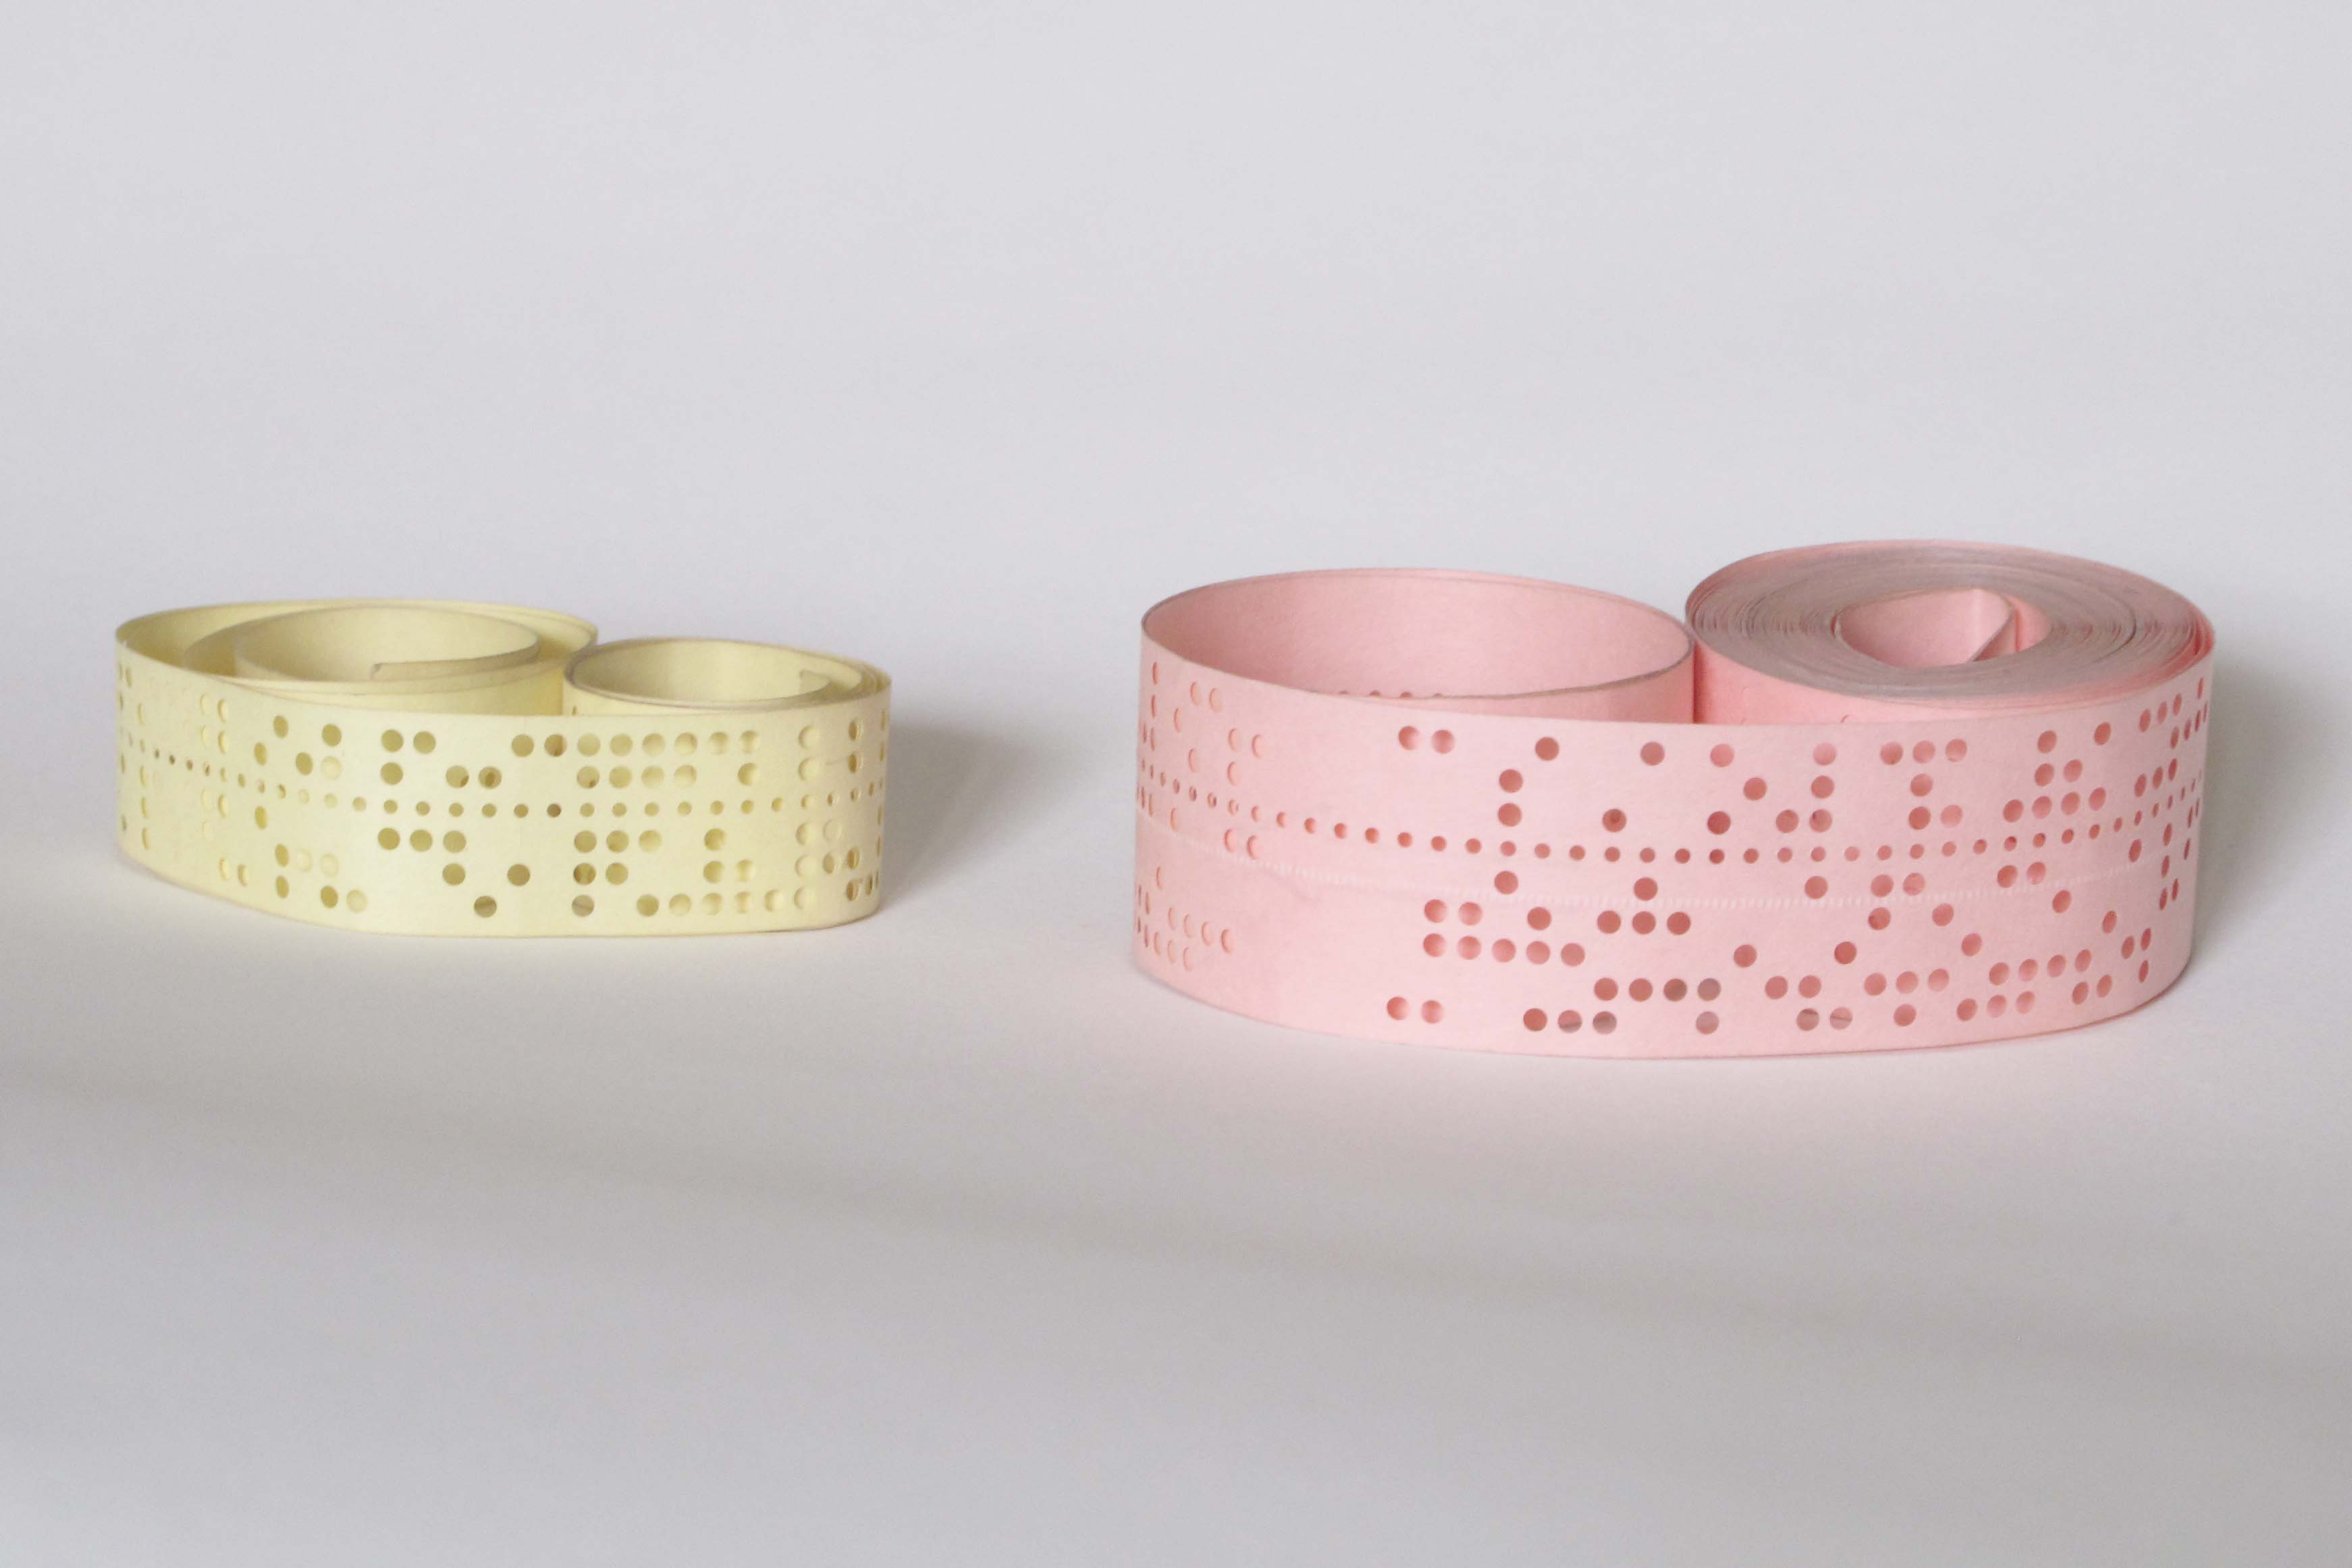
\includegraphics[scale=0.5]{PerforatedTape}
\caption{Perforated tape, utilized to store bits as punched holes}
\end{figure}

However, this system had a vulnerability which the One-Time Pad solved: In Vernam's original method, the perforated tape was not exchanged after it had completed one cycle; instead, it was looped around continuously, often being used to encrypt multiple different messages.

This made the entire system vulnerable. The re-usage of the key meant that the resulting ciphertext suffered from a so-called known-plaintext vulnerability \cite{HutSix}. This means that, if a plaintext and its corresponding ciphertext are captured, the key utilized to generate the ciphertext can be derived from them. This is not an issue if the key is exchanged each time a new message is encrypted. However, if the key of any Vernam cipher machine was compromised through a known-plaintext attack, any further intercepted ciphertexts could be decrypted.

\begin{figure}[H]
\centering
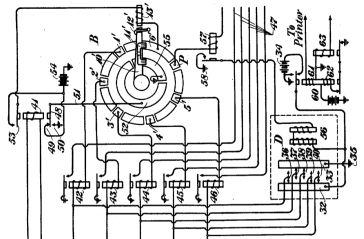
\includegraphics[scale=1]{VernamCipher.jpg}
\caption{An image from Vernam's famous "Secret signaling system" patent of 1919.}
\end{figure}    

\section{Method used}
%This section, especially the practical example, is the most important part of the chapter.
In the following section, the utilized method will be clarified through usage of an example. In this example, the message \textit{"cryptography"} will first be encrypted by its sender, sent to its intended recipient, and finally decoded by the recipient.

\subsection{Generation of the random key}
In order to encrypt the plaintext, a key must first be generated. This key will be utilized to encrypt the plaintext through the usage of modular addition, turning it into the ciphertext.

This key must fulfil some crucial criteria \cite{MilsElectronic}. Foremost, the length of the key (the amount of  characters contained within it) must be equivalent to or greater than the length of the plaintext; otherwise, it is not possible to perform any encryption (using the OTP). Secondly, the key must be generated randomly. This is mainly due to the fact that a randomly generated key makes frequency analysis\cite{FrequencyAnalysis}, the form of cryptanalysis most commonly used to break classical ciphers, impossible.

The key consists of numbers. Usually, when the plaintext is made up of Latin letters, the numbers range between 0 and 25. The key can be converted into Latin letters through the same method applied to the plaintext outlined in the following chapter, however, this is not necessary, although the key is often transported in the form of text.

As the message being encrypted in this example has 12 characters, the key must also posses at least 12 characters. For the sake of this example, the key \textit{"sytruifgnihm"} will be utilized.

\subsection{Modular addition of the key and plaintext}
%unsure if a picture explaining modular addition and subtraction is needed, or if the provided explanation suffices?			
Next, the ciphertext is created through modular addition of the key and the plaintext. This can be applied not only to a message consisting of alphabetical characters, but also to any sequence of bits. If the plaintext consists of a message made up of alphabetical characters, the plaintext and the key are added using arithmetic referred to as \textit{"addition modulo 26"}. The correct mathematical notation for modular arithmetic is $(a+b)\:mod\:c$, where c is referred to as the \textit{modulus}, which is the value that cannot be passed nor reached in modular addition. In order to perform modular addition, the variables a and b are first added, after which they are divided by the modulus c, up to an integer. The resulting remainder r is the final result of the operation.

Before the modular addition of the plaintext and the key can begin, each character (of the plaintext as well as of the secret key, in the case that the key was generated as a string of Latin letters instead of as a sequence of numbers) must be converted to a number, corresponding to it's position in the Latin alphabet:

\begin{figure}[H]
\centering
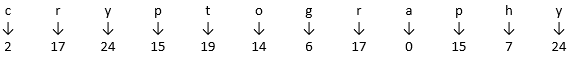
\includegraphics[scale=1]{Table1.PNG}		
\end{figure}
%Do these tables suffice in aiding understanding the example, or 		                                             should I include more "graphical" explanations as well?

As the key was also generated in the form of characters, it too must be converted to a sequence of numbers:

\begin{figure}[H]
\centering
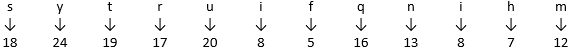
\includegraphics[scale=1]{Table2.PNG}
\end{figure}

Afterwards, the key and the plaintext are added together utilizing modular addition. Of course, all operations below are performed in \textit{mod 26}. Finally, the resulting numbers are converted to the character to which they correspond in the Latin alphabet. The resulting sequence of characters is referred to as the ciphertext.

\begin{figure}[H]
\centering
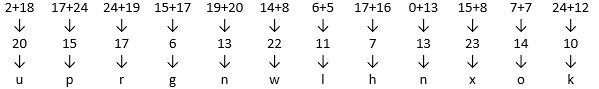
\includegraphics[scale=1]{Table3.PNG}
\end{figure}

\subsection{decoding of the ciphertext using the key}
Assuming the message has been delivered to the intended recipient, who must hold a copy of the secret key (which, as OTP is a symmetrical cryptographical method, is identical to the one utilized to create the ciphertext), the recipient can now decode the ciphertext in order to view the plaintext.

Since the ciphertext was created through the modular addition of the plaintext and the key, the recipient can utilize modular subtraction in order to view the plaintext. In order to do this, the recipient must subtract the key from the ciphertext in modulo 26, and convert the resulting numbers to Latin characters.  However, it is now also necessary for the numbers not to become negative. Fortunately, this is also made possible by modular arithmetic, as the values simply loop back around from 0 as well. Once again, all below operations are in \textit{mod 26}.

\begin{figure}[H]
\centering
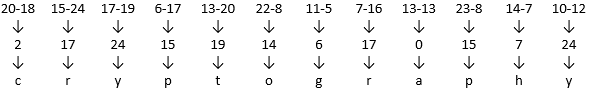
\includegraphics[scale=1]{Table4.PNG}
\end{figure}

Now, the message's journey is complete, having passed from plaintext into ciphertext, being transported to its intended recipient in the form of ciphertext, and finally being decoded and read by its recipient. 

\section{Perfect secrecy: Information-theoretical security}
An important characteristic of OTP is that the ciphertext convey no information at all in regards to the plaintext; this means that it is not possible to garner any information about the key nor the plaintext if one is in possession of the ciphertext \cite{PerfectSecrecy} \cite{HandbookOfAppliedCryptography}.

From this, two other important characteristics of a cryptographical system with perfect secrecy can be derived. Firstly, perfect message indistinguishability. This means that, even if you are provided with multiple different plaintexts and one ciphertext, it is impossible to assign any one plaintext to the provided ciphertext. Secondly, if the key is the same length as the plaintext (as is the case in OTP), then there exists a key for every possible encryption from plaintext to ciphertext. This means that any plaintext can be converted to any ciphertext, making it impossible to determine the key without access to both the plaintext and the ciphertext. This is referred to as perfect key ambiguity.		%This paragraph was difficult for me to summarize well.

Although many believe that the ciphertext does provide information about the plaintext, namely its length, this can easily be solved through padding, where characters of no importance to the plaintext are added to it before encryption \cite{HutSix}.

\subsection{mathematical proof}
%This is the section which was most difficult for me to write; I opted to present a more simplified explanation of %Shannons proof without the use of probability theory.
%Should I Include the probability Theory or is it better to keep it simple for the reader?
In 1949, Shannon proved the perfect secrecy of OTP by using probability theory \cite{ShannonOTP}. To be precise, he proved that, in order to achieve perfect secrecy, the key must possess at least the same length as the plaintext; one of the key characteristics of OTP. If this is the case, then an attacker cannot determine the plaintext given the ciphertext, even with access to infinite computational capacity; a "brute-force attack" is impossible.

A simplified method of presenting this proof is as follows:

If the attacker does indeed possess infinite computational capacity, he can generate every possible key which could have been used to generate the ciphertext, and he can then generate every possible plaintext (each of which will correspond to the given ciphertext and one of the generated keys).

It follows that, if the ciphertext was $m$ bits long, there would be $2^m$ possible keys (or, in the case that the plaintext and ciphertext consist of Latin characters, $26^m$ possible keys). This is because a bit can possess the value of either 0 or 1, meaning that each individual bit of the key has two possible values. As The entire key possesses m bits, each cell must be multiplied by the following cell in order to obtain the total number of possible keys. In the case that the key consists of Latin characters, however, each cell possess 26 possible values (ranging from 0 to 25); therefore, the total number of possible keys would be $26^m$.

If the possible amount of keys that the attacker can generate is equal to $2^m$, and the attacker can generate one possible plaintext for each key, that means that the amount of plaintexts which the attacker can generate is also equal to $2^m$ (or, once again, in the case of Latin characters, equal to $26^m$ plaintexts).

This amount, $2^m$, is equal to the amount of possible bit sequences of the length m; therefore, the attacker cannot possibly eliminate any one possible plaintext of the length m, meaning that he cannot garner any information from the ciphertext on its own. This fulfils the requirements of perfect secrecy.

\subsection{Why can only OTP achieve perfect secrecy?}
%Not sure if this information warrants its own section or if I should merge it with the above one
From the above proof, it can be concluded that, in order for the elimination of any possible plaintext to be impossible (rendering a brute-force attack impossible), the key must possess at least the same length as the plaintext. Also, the individual bits of the must not be dependant on one another. These conditions are only fulfilled by OTP.  

\section{Issues with OTP}
%I had just one sentence here, but felt it appeared strange to just have one sentence and opted to leave it blank.
\subsection{True randomness in generating the key}
One of the most important aspects of the utilized key is that it must be completely random (see 1.2.1). However, generating a random sequence of numbers or letters is no trivial task. In fact, most random number generation functions of even modern programming languages are not adequately random for use in cryptography. This is especially difficult for computers, considering that a computer is, in essence, designed to follow a set of predictable instructions as quickly as possible.

Therefore, in order to generate a sufficiently random key, it is preferable to utilize hardware random number generators, for example by utilizing a true random noise source \cite{MilsElectronic}. One such example is the key generator built by mils electronic, where a set of parallel ring oscillators are sampled. Because the oscillation speed of each ring is influenced by random factors such as local variations in temperature and voltage.

\begin{figure}[H]
\centering
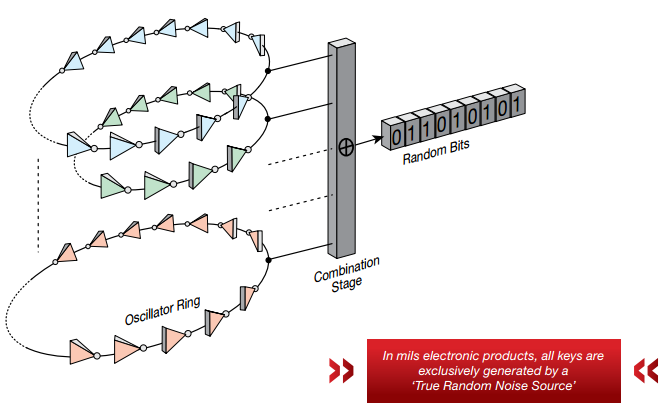
\includegraphics[scale=0.75]{MilsElectronic.PNG}
\caption{A hardware random number generator with sufficient randomness to be utilized in the generation of one-time pads.}
\end{figure}

\subsection{Secure distribution of the key itself}
The main issue in regards to OTP is that, while it posses perfect security, therefore solving the issue of safely transmitting the ciphertext, the problem instead becomes how to securely transmit the key to the intended recipient of the encrypted message.

Therefore, in order to ensure that the plaintext cannot be accessed by any party other than its intended recipient, the complete security of the transmittal of the key must also be ensured.

However, if the communicants already possess a method by which the key can be transmitted with infallible security, then it stands to reason that the plaintext itself could just as well be submitted through the same channel, considering that it has the same number of bytes (or characters) as the key. So, the problem of securely transmitting the plaintext has simply been transferred to the problem of securely transmitting the key.

One method of mitigating this issue is to first send one very long key, which can then be used for multiple messages in the future. Using this method, only one secure transmission has to be made in order to ensure the security of multiple transmissions. 

\subsection{Secure disposal of a utilized key}
%Once again, not entirely sure if this warrants its own section or if it should be merged into the above section.
After a key has been fully utilized, it has to be disposed of securely, in order to prevent any information from being compromised in the future, which is possible should the key continue to exist. Therefore, it is necessary to completely eradicate the entirety of the key. If the key was stored on a digital media, such as a USB drive or HDD, the only completely secure method of disposal is considered to be complete incineration. 

\printbibliography

\end{document}

